\section{Durchführung}
\label{sec:Durchführung}
\subsection{Lasergranulation}
Um den Schwellenstrom zwischen LED (light emitting diode) und Laserlicht zu bestimmen,
wird der Effekt der Lasergranulation verwendet.
Lasergranulation tritt auf, wenn Laserlicht auf eine unebene Fläche trifft 
und dort reflektiert wird.
Nach dem Huygen'schen Prinzip entsteht dabei an jeder Unebenheit eine neue Kugelwelle.
Trift nun Monochromatisches Licht auf diese Streuzentren entsteht ein zufälliges Interferenzmuster,
welches als körnige Lichtflecke zu erkennen sind.
Um diesen Schwellenstrom zu bestimmen wird eine unebene Oberfläche in den Laserstrahl gebracht (vgl. Abbildung \eqref{fig:Lasergranulation}).
\begin{figure}[h]
    \centering
    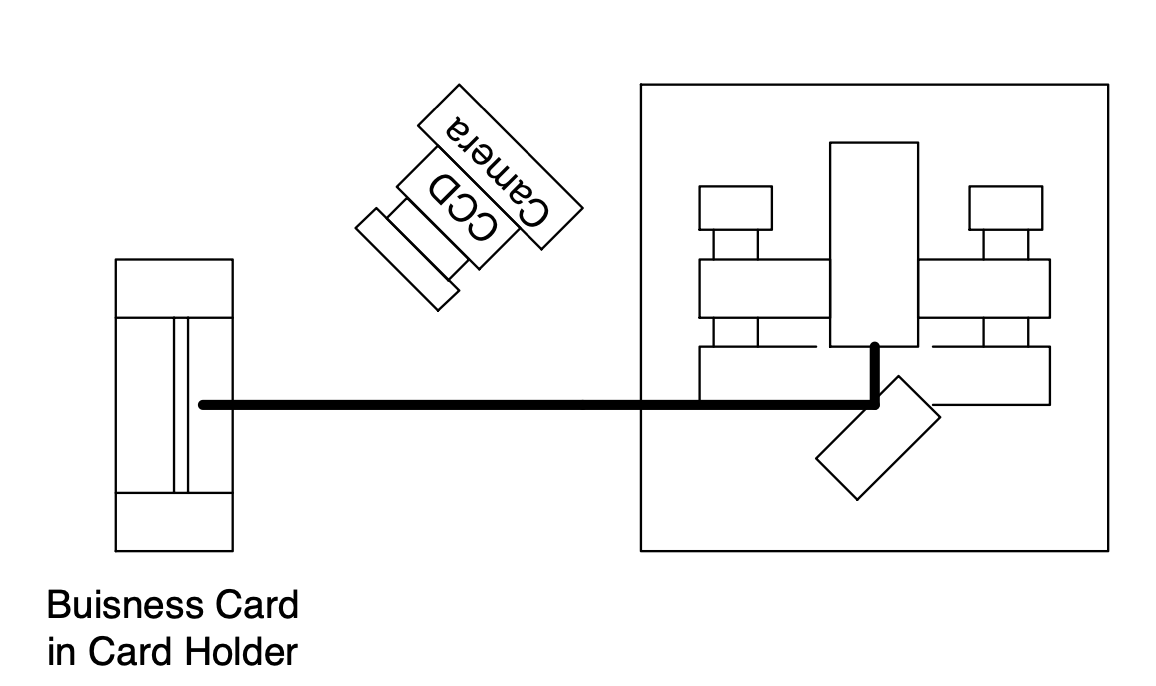
\includegraphics[width=0.7\textwidth]{abb/aufbau1.png}
    \caption{Aufbau Lasergranulation \cite{aufbau}}
    \label{fig:Lasergranulation}
\end{figure}
Strom und Winkel des Lasers werden so eingestellt,
dass Lasergranulation beim kleinstmöglichen Strom auftritt.
Die CCD Kamera dient als Detektor für das Infrarotlicht,
da dieses mit bloßen Auge nicht zu erkennen ist.

\subsection{Aufnahme des Transmissionsspektrums von Rubidium}

